\chapter{Opis projektnog zadatka}
		
		Cilj ovog projekta je razviti programsku podršku za stvaranje web aplikacije "\textit{StreetPatrol}". Ideja aplikacije je ponuditi običnim građanima jednostavan i efikasan način prijave oštećenja javnih površina i cesta u gradu te dobivanje povratnih informacija o konkretnom oštećenju i njihovoj prijavi. 
		
		Građani će svojim djelovanjem putem aplikacije unaprjeđivati kvalitetu života u svojoj zajednici. Svojim prijavama, koje će biti javno dostupne, građani će poticati gradske urede da saniraju prijavljena oštećenja. Aplikacija će također pomoći gradskim uredima u obavljanju svojih zadaća. Naime, preko aplikacije uredi će imati puno bolji uvid u probleme koji postoje u zajednici. Zahvaljujući aplikaciji uredi će moći brže i kvalitetnije reagirati na probleme u zajednici.
		
		Slične aplikacije već postoje u Hrvatskoj. Tako primjerice Grad Rijeka na svojim stranicama nudi mogućnost prjave raznih prekršaja i oštećenja (\url{https://gov.rijeka.hr/zahtjevi-i-obrasci/komunalna-djelatnost-i-prijava-komunalnog-nereda/prijave-ostecenja-nereda-ili-nepropisnog-parkiranja/383}). Njihova stranica nudi mogućnost prijave u 4 kategorije. Neke prijave se podnose putem obrazaca, neke samo telefonskim putem, a za neke su ponuđene i specijalne stranice. Tako primjerice za prijavu većine problema, ali i za podnošenje pohvala, Grad Rijeka nudi web aplikaciju \textit{Gradsko oko} (\url{http://rijeka.oko.hr/}) dostupnu i u mobilnoj verziji. Aplikacija nudi mogućnost podnošenja i pregleda prijava putem interaktivne karte. Prijave su kategorizirane po grupama i klasifikacijama. Prilikom pregleda se mogu filtrirati po vremenu i kategorijama. Prijave i pregled prijava su dostupne samo prijavljenim korisnicima te svaka prijava mora biti odobrena od strane administratora.
		
		\begin{figure}[H]
			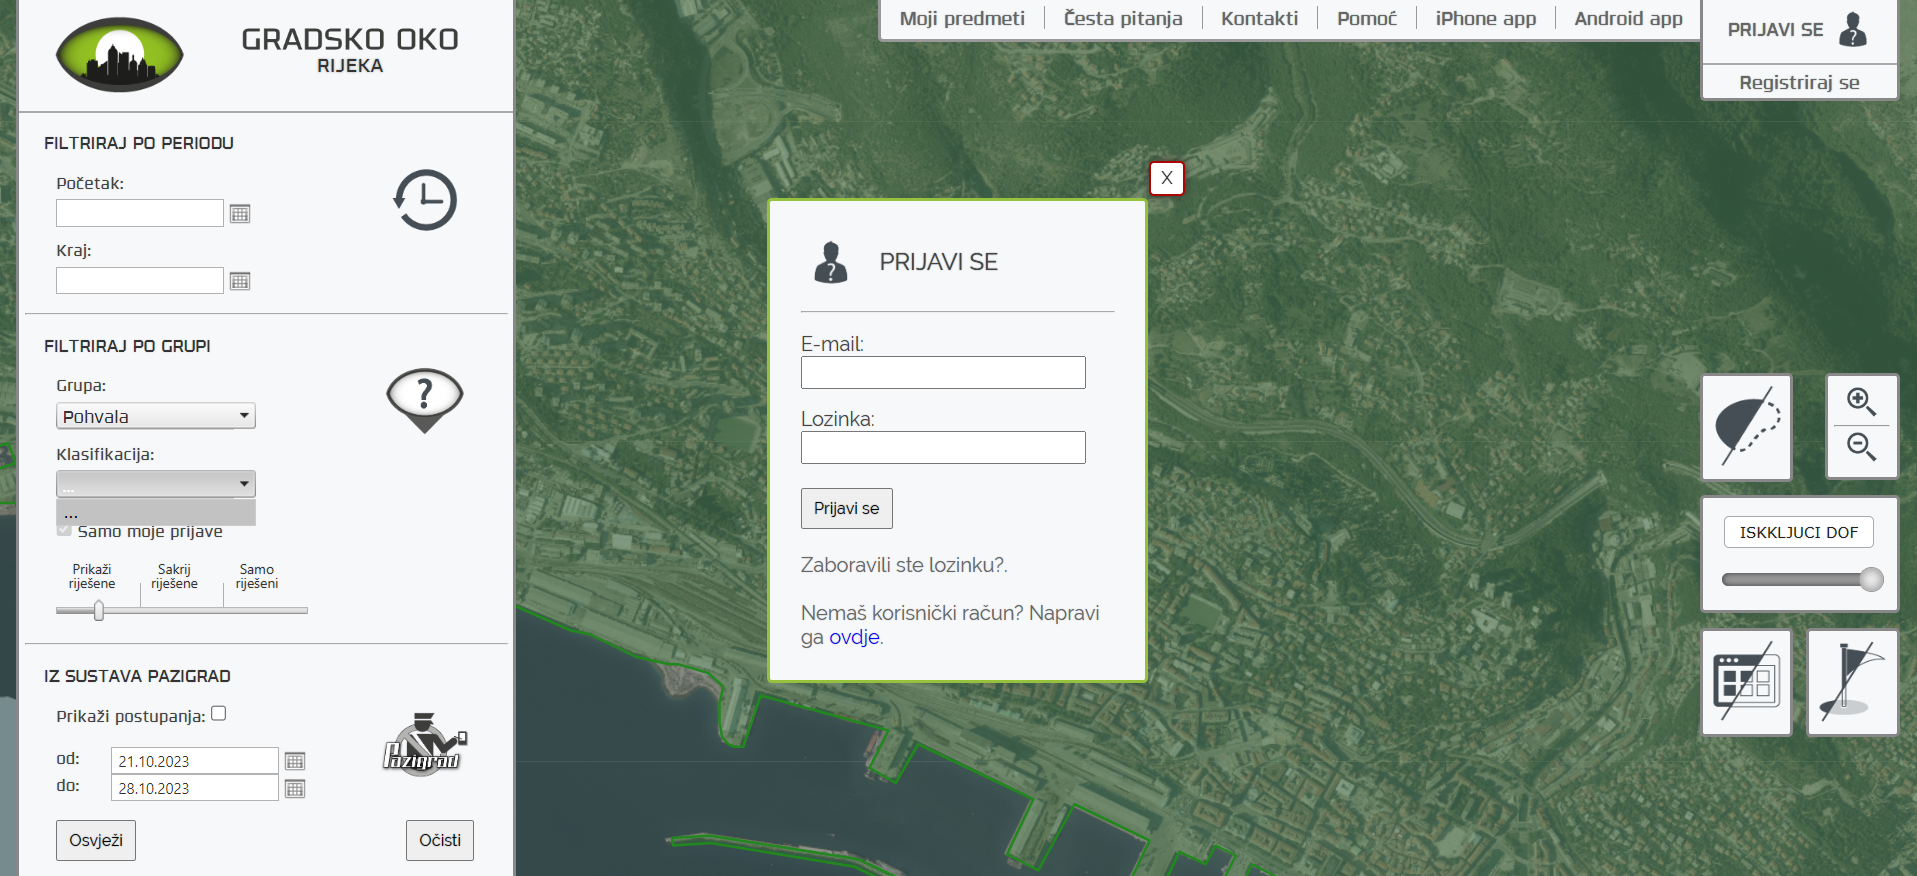
\includegraphics[width=\textwidth]{slike/GradskoOko.PNG}
			\caption{Aplikacija \textit{Gradsko oko} Grada Rijeke}
			\label{fig:gradskooko} %label mora biti drugaciji za svaku sliku
		\end{figure}
		
		\underbar{Građani} aplikaciju mogu koristiti kao registrirani i kao neregistrirani korisnici. Na naslovnoj stranici građanima su ponuđene opcije podnošenja nove prijave, pregleda postojećih prijava i pregled statistike prijava. Registrirani građani također imaju opciju pregleda svojeg profila dok neregistrirani građani imaju mogućnost registracije, tj. izrade profila odnosno prijave, ako već imaju izrađeni profil.
		
		Neregistrirani korisnik se može registrirati te prilikom registracije mora navesti sljedeće informacije:
		\begin{packed_item}
			\item ime
			\item prezime
			\item email adresa
			\item lozinka
		\end{packed_item}  
		Prijavljeni korisnici prilikom pregleda svojeg profila mogu vidjeti prije navedene podatke o sebi koje mogu i izmjeniti. Također imaju pregled nad svim prijavama koje su podnesli kroz aplikaciju. Prikazana im je i kratka statistika prijava (broj prijava, broj riješenih prijava, broj prijava na čekanju i u procesu rješavanja). 
		
		Građanima se prilikom podnošenja nove prijave otvara obrazac koji je potrebno ispuniti. Prijava sadrži naslov koji definira oštećenje. Slijedi kratak opis u kojem korisnik detaljnije opisuje oštećenje u slobodnoj formi. Korisnik dalje prilaže geografski položaj oštećenja koje se prijavljuje. Geografski položaj se prilaže odabirom položaja na karti koja će se moći otvoriti prilikom ispunjavanja obrasca ili upisivanjem adrese na kojoj se nalazi oštećenje. Također korisnik će moći priložiti geografski položaj automatski preko svoje trenutne lokacije. Korisniku se nudi opcija da uz prijavu priloži fotografije oštećenja. Ukoliko korisnik priloži fotografije, aplikacija će pokušati iz njih izvući podatke o lokaciji te ih ponuditi korisniku kao lokaciju oštećenja. Korisnik u prijavi mora odabrati kategoriju oštećenja. Time korisnik indirektno odabire gradski ured nadležan za konkretan problem. Prilikom opisivanja oštećenja aplikacija će pokušati sama zaključiti kojoj kategoriji oštećenje pripada te će istu predložiti korisniku. Također, ako u sustavu već postoji slična nedavna prijava na istoj lokaciji aplikacija će predložiti korisniku već postojeću prijavu i ponuditi mu da svoju prijavu nadoveže na već postojeću. Nakon podnošenja prijave aplikacija korisniku daje jedinstveni kod podnesene prijave koja služi za praćenje te prijave preko same aplikacije. Prijavljeni korisnici će također primati obavijesti o svojoj prijavi preko emaila.
		
		Za pregled postojećih prijava korisniku je na naslovnoj stranici priložena interaktivna karta s označenim prijavama na njoj. Prijave se mogu dodatno filtrirati po vremenu podnošenja prijave, statusu, kategoriji oštećenja i nadležnom gradskom uredu. Korisnik također može pretraživati prijave po jedinstvenom kodu prijave. Na taj način svaki korisnik može pregledavati svoje prijave na aplikaciji. Odabirom neke prijave prikazuju se podaci iz podnesenog obrasca o odabranoj prijavi. Također se prikazuje status prijave (\textit{na čekanju}, \textit{u procesu rješavanja}, \textit{riješena}), broj prijava koje su vezane za ovu prijavu, odnosno prijava za koju je vezana ova prijava. Prijavljeni korisnici također vide svoje prijave na pregledu svojeg profila. Prijave koje su riješene mogu se pregledati jedino preko njihovog koda ili preko pregleda korisničkog profila kod registriranih korisnika. U drugim slučajevima takve prijave nisu više dostupne za pregled.
		
		Prikaz statistike prijava nudi filtriranje podataka po vremenu podnošenja prijave, kategoriji oštećenja i nadležnom gradskom uredu. Za odabrane parametre aplikacija prikazuje:
		\begin{packed_item}
			\item ukupan broj podnešenih prijava
			\item broj prijava sa statusom \textit{na čekanju} i njihov udio
			\item broj prijava sa statusom \textit{u procesu rješavanja} i njihov udio
			\item broj prijava sa statusom \textit{riješena} i njihov udio
			\item prosječan broj podnesenih prijava u danu
			\item prosječan broj dana koji prijava provede na čekanju
			\item prosječan broj dana za vrijeme kojih je prijava u procesu rješavanja
		\end{packed_item}
		
		\underbar{Djelatnici gradskog ureda} se obavezno u sustav prijavljuju preko profila gradskog ureda. Djelatnici na svojoj naslovnoj stranici imaju 3 liste prijava, jedna za svaku vrstu statusa: novopristigle, one u procesu rješavanja i riješene prijave. Djelatnici ureda imaju isključivo pristup prijavama za probleme za koje je nadležan njihov ured. Ostale prijave djelatnicima nisu vidljive.
		
		Sustav nudi mogućnost registracije novih gradskih ureda. U tom slučaju kod stranice za registraciju potrebno je odabrati opciju registracije gradskog ureda. Aplikacija tada prikazuje obrazac za koji je potrebno navesti:
		\begin{packed_item}
			\item ime gradskog ureda
			\item email adresa gradskog ureda
			\item lozinka za račun gradskog ureda
			\item jedna ili više kategorija koje će novi gradski ured pokrivati
		\end{packed_item}
		Nakon podnošenja popunjenog obrasca sustav provjerava valjanost podataka. Ako su podaci valjani, otvara se naslovna stranica za djelatnike gradskih ureda. U suprotnom se javlja greška i vraća se stranica za registraciju.
		
		Djelatnici pregledavaju pristigle prijave i stavljaju ih u proces rješavanja. Time prijave prelaze u listu prijava u procesu rješavanja i mijenjaju svoj status. Aplikacija u tom slučaju automatski šalje mail prijavitelju ako se radi o registriranom korisniku.
		
		Kada neka prijava bude riješena, djelatnik prijavi mijenja status u \textit{riješena}. Prijava prelazi u za to predviđenu listu te aplikacija šalje mail  prijavitelju ako se radi o registriranom korisniku.
		
		Djelatnik ima mogućnost objedinjavanja prijava. Naime, ako se pristigla prijava referira na problem za koji već postoji prijava, djelatnik može grupirati te prijave. U tom slučaju se najstarija od tih prijava tretira kao glavna prijava, a ostale prijave postaju nadovezane na tu prijavu. Aplikacija u tom slučaju šalje prikladnu obavijest registriranim korisnicima čije su prijave sada nadovezane na glavnu prijavu.
		
		Ako procijeni da je pristigla prijava poslana na krivi ured, djelatnik ima mogućnost proslijediti prijavu uredu koji je zapravo nadležan za pristiglu prijavu. Korisniku koji je podnio prijavu se u tom slučaju šalje prikladna obavijest putem maila ako je taj korisnik registriran.
		
		Slično, ako procijeni da pristigla prijava uopće nije valjana, djelatnik ima mogućnost odbaciti prijavu. U tom slučaju se prijava arhivira u bazi podataka ali se više ne koristi. Korisnik koji je podnio prijavu dobiva prikladnu obavijest putem maila ako je registriran.
		
		Kao i kod običnih korisnika, djelatnici ureda mogu pregledavati prijave preko karte. Također mogu pregledavati statistiku prijava kao i obični korisnici, uz restrikciju na prijave vezane na njihov ured, kao što je prije navedeno.
		
		Aplikacija je napravljena tako da podržava višejezičnost. Aplikacija podržava hrvatski i engleski jezik.
		
		Aplikacija je napravljena na primjeru Grada Zagreba, prvenstveno u smislu da će aplikacija predviđati postojanje gradskih ureda relevantnih za ovu problematiku kakvi su ustrojeni u Zagrebu. Konkretno, aplikacija predviđa postojanje sljedećih ureda:
		\begin{packed_item}
			\item Gradski zavod za zaštitu spomenika kulture i prirode - za oštećenja na spomenicima kulture i prirode
			\item Gradski ured za mjesnu samoupravu, promet, civilnu zaštitu i sigurnost - za oštećenja na komunalnoj infrastrukturi vezanoj za oborinske vode, površinama javne namjene, u gradskim parkovima i zelenim površinama, cestama
			\item Gradski ured za obnovu, izgradnju, prostorno uređenje, graditeljstvo i komunalne poslove - za oštećenja na zgradama, komunalne probleme
		\end{packed_item}
		Kao što je već i navedeno, aplikacija će pružati mogućnost dodavanja novih ureda kako bi se lakše mogla prilagoditi promjenama u ustrojstvu ureda. Također, sve karte na aplikaciji će inicijalno prikazivati područje Grada Zagreba. Prijavljivanja oštećenja izvan tog područja neće biti moguća, tj. takva lokacija će se smatrati nevažećom i takva prijava se neće moći podnesti.
		
		Uz male preinake moguće je prilagoditi aplikaciju da pruža istu potporu građanima nekog drugog grada ili općine, bilo u Hrvatskoj ili nekoj drugoj zemlji. Aplikacija bi se mogla skalirati i na veće jedinice lokalne samouprave kao što su županije, s obzirom da obično imaju sličan ustroj ureda i slične nadležnosti kao i gradovi. Ako se ideja skalira još više, aplikacija bi mogla pružati uslugu korisnicima cijele regije (npr. Slavonija, Dalmacija, Središnja Hrvatska) ili čak čitave države. U tom slučaju u aplikaciji bi bilo potrebno dodati mogućnost prepoznavanja nadležne jedinice lokalne samouprave prije predlaganja nadležnog ureda za konkretan problem. Takvo ponašanje bi se moglo implementirati uz malo prerađivanja i korištenje već postojećih funkcionalnosti aplikacije. Generalno gledano, aplikacija bi se mogla skalirati tako da pruža uslugu korisnicima nadnacionalnoj razini, primjerice na području cijele Europske Unije. Ponašanje aplikacije bi zapravo bilo isto uz potrebe skaliranja funkcionalnosti prepoznavanja nadležnih administrativnih jedinica na nadnacionalnoj razini. U tom slučaju aplikacija svakako mora pružati mogućnost prikaza na jeziku svake države u kojoj pruža uslugu. Glavna prepreka u ovakvoj implementaciji bi bila potreba za značajnijom infrastrukturalnom podrškom, prvenstveno u obliku velikih poslužitelja koji mogu obrađivati puno zahtjeva i pohranjivati velike količine podataka. Također, aplikacija bi na toj razini zahtjevala dobru suranju i koordinaciju velikog broja institucija u više različitih država što može biti zahtjevno.
		
		\eject
		
		\section{Primjeri u \LaTeX u}
		
		\textit{Ovo potpoglavlje izbrisati.}\\

		U nastavku se nalaze različiti primjeri kako koristiti osnovne funkcionalnosti \LaTeX a koje su potrebne za izradu dokumentacije. Za dodatnu pomoć obratiti se asistentu na projektu ili potražiti upute na sljedećim web sjedištima:
		\begin{itemize}
			\item Upute za izradu diplomskog rada u \LaTeX u - \url{https://www.fer.unizg.hr/_download/repository/LaTeX-upute.pdf}
			\item \LaTeX\ projekt - \url{https://www.latex-project.org/help/}
			\item StackExchange za Tex - \url{https://tex.stackexchange.com/}\\
		
		\end{itemize} 	


		
		\noindent \underbar{podcrtani tekst}, \textbf{podebljani tekst}, 	\textit{nagnuti tekst}\\
		\noindent \normalsize primjer \large primjer \Large primjer \LARGE {primjer} \huge {primjer} \Huge primjer \normalsize
				
		\begin{packed_item}
			
			\item  primjer
			\item  primjer
			\item  primjer
			\item[] \begin{packed_enum}
				\item primjer
				\item[] \begin{packed_enum}
					\item[1.a] primjer
					\item[b] primjer
				\end{packed_enum}
				\item primjer
			\end{packed_enum}
			
		\end{packed_item}
		
		\noindent primjer url-a: \url{https://www.fer.unizg.hr/predmet/proinz/projekt}
		
		\noindent posebni znakovi: \# \$ \% \& \{ \} \_ 
		$|$ $<$ $>$ 
		\^{} 
		\~{} 
		$\backslash$ 
		
		
		\begin{longtblr}[
			label=none,
			entry=none
			]{
				width = \textwidth,
				colspec={|X[8,l]|X[8, l]|X[16, l]|}, 
				rowhead = 1,
			} %definicija širine tablice, širine stupaca, poravnanje i broja redaka naslova tablice
			\hline \SetCell[c=3]{c}{\textbf{naslov unutar tablice}}	 \\ \hline[3pt]
			\SetCell{LightGreen}IDKorisnik & INT	&  	Lorem ipsum dolor sit amet, consectetur adipiscing elit, sed do eiusmod  	\\ \hline
			korisnickoIme	& VARCHAR &   	\\ \hline 
			email & VARCHAR &   \\ \hline 
			ime & VARCHAR	&  		\\ \hline 
			\SetCell{LightBlue} primjer	& VARCHAR &   	\\ \hline 
		\end{longtblr}
		

		\begin{longtblr}[
				caption = {Naslov s referencom izvan tablice},
				entry = {Short Caption},
			]{
				width = \textwidth, 
				colspec = {|X[8,l]|X[8,l]|X[16,l]|}, 
				rowhead = 1,
			}
			\hline
			\SetCell{LightGreen}IDKorisnik & INT	&  	Lorem ipsum dolor sit amet, consectetur adipiscing elit, sed do eiusmod  	\\ \hline
			korisnickoIme	& VARCHAR &   	\\ \hline 
			email & VARCHAR &   \\ \hline 
			ime & VARCHAR	&  		\\ \hline 
			\SetCell{LightBlue} primjer	& VARCHAR &   	\\ \hline 
		\end{longtblr}
	


		
		
		%unos slike
		\begin{figure}[H]
			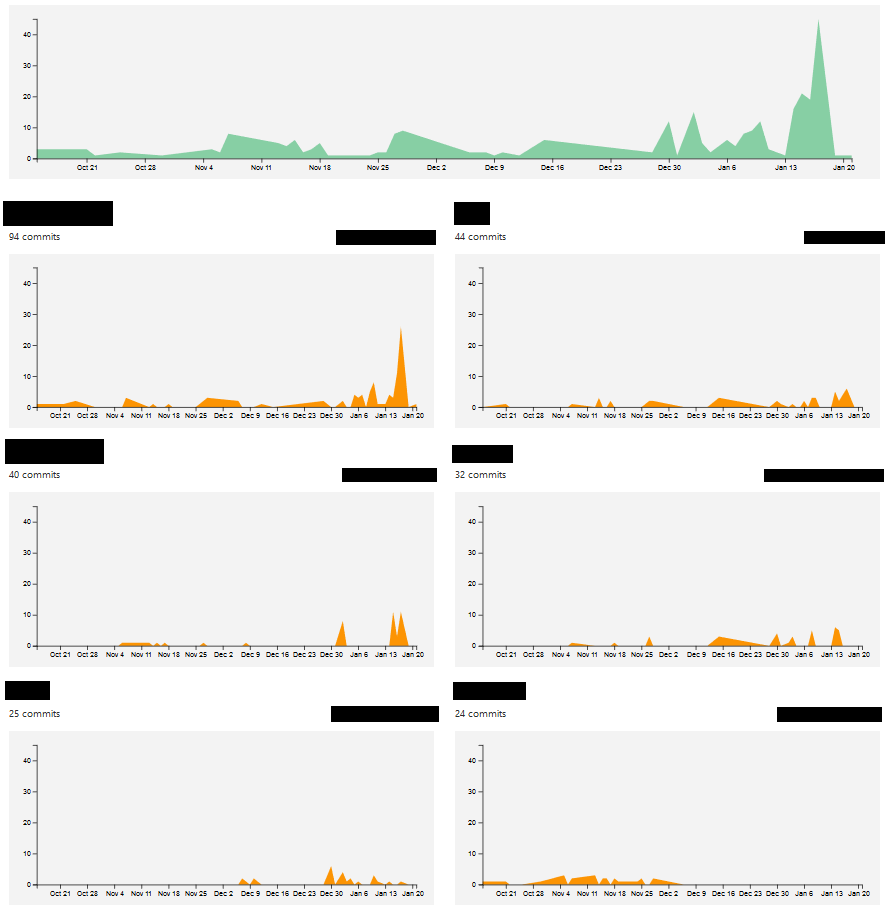
\includegraphics[scale=0.4]{slike/aktivnost.PNG} %veličina slike u odnosu na originalnu datoteku i pozicija slike
			\centering
			\caption{Primjer slike s potpisom}
			\label{fig:promjene}
		\end{figure}
		
		\begin{figure}[H]
			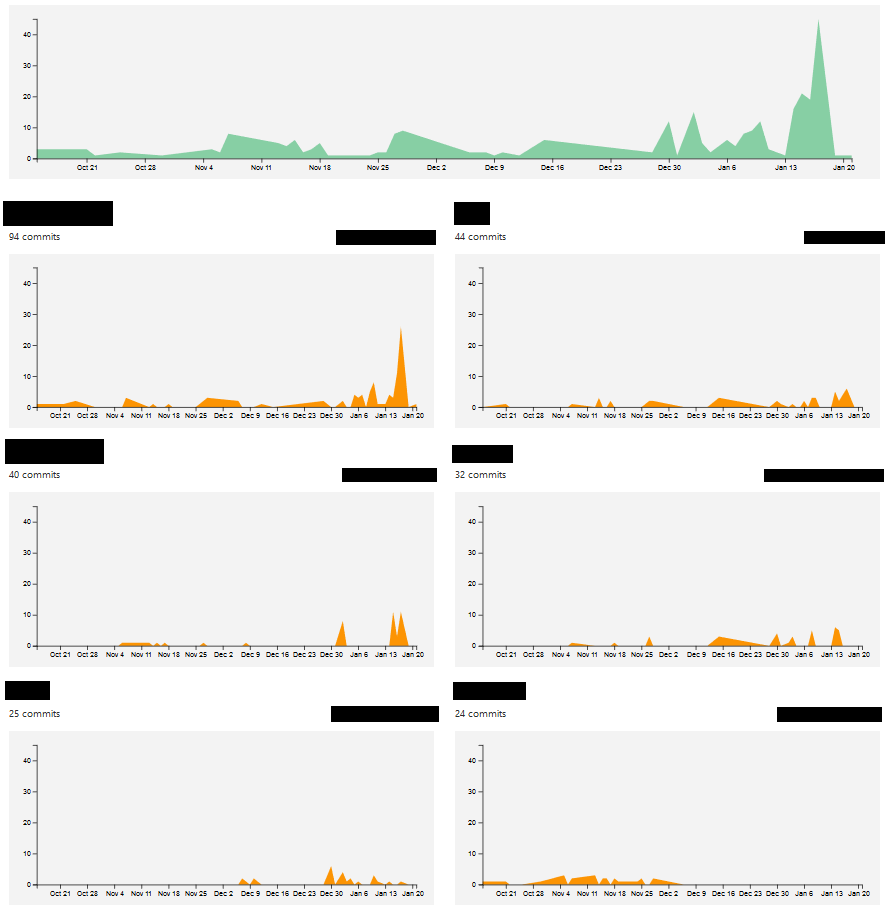
\includegraphics[width=\textwidth]{slike/aktivnost.PNG} %veličina u odnosu na širinu linije
			\caption{Primjer slike s potpisom 2}
			\label{fig:promjene2} %label mora biti drugaciji za svaku sliku
		\end{figure}
		
		Referenciranje slike \ref{fig:promjene2} u tekstu.
		
		\eject
		
	